\documentclass{mwart}

\usepackage{polski} % Pozwala na użycie polskiego. Ustawia między innymi fontenc na T1
\usepackage[utf8]{inputenc} % Informuje o kodowaniu
\usepackage{xcolor} % Definicje kolorów

\usepackage{graphicx}
\graphicspath{ {./Obrazy/} }

\usepackage{float} % Pozycjonowanie figur

\usepackage{listings} % Listingi kodu
\lstset{basicstyle=\ttfamily,
  showstringspaces=false,
  commentstyle=\color{gray},
  keywordstyle=\color{blue}
}

\usepackage{textcomp} % Znaki specjalne takie jak ~

\title{Laboratorium sieci komputerowych - c2 \\ Konfiguracja interfejsów sieciowych}
\author{Krzysztof Dąbrowski gr. 3}
\date{\today}

\begin{document}
\maketitle{}
\tableofcontents{}
%\newpage

\section{Pierwsze zajęcia}
Celem pierwszej części zajęć c2 było odwzorowanie schematu sieci na stacji roboczej. By to osiągnąć trzeba było wykreować maszyny wirtualne oraz odpowiednie interfejsy sieciowe.

\begin{figure}[h]
    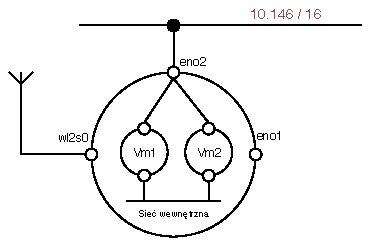
\includegraphics[width=0.80\textwidth]{schemat}
    \centering
    \caption{Schemat sieci do wykreowania}
    \label{fig:schemat}
\end{figure}

\subsection{Zbadanie lokalnych interfejsów}
Dzięki poleceniu \texttt{ifconfig} można uzyskać informacje o interfejsach gospodarza. Uzyskanie w tens sposób nazwy interfejsów zostały naniesione na schemat %\ref{fig:schemat}.

\subsection{Kreacja wirtualnych maszyn}
W celu automatyzacji tworzenia maszyn wirtualnych napisałem prosty skrypt konfiguracyjny.

\lstinputlisting[language=bash]{./Skrypty/c2}

Możliwe było również wyszukanie \textbf{gotowego skryptu} i modyfikacja go do własnych potrzeb. W tym celu można było skorzystać z programu \texttt{grep}. \\
Przykład wyszukania skryptów związanych z Virtual Box: \texttt{grep -iRl "VboxManage" /usr/local/zetis/bin}

\section{Drugie zajęcia}
Celem drugich zajęć było wygenerowanie pojedynczej wirtualnej maszyny oraz konfiguracja wirtualnych interfejsów sieciowych wewnątrz tej maszyny.

\subsection{Schemat struktury sieci}

\subsection{Generacja maszyny}
Do utworzenia maszyny zmodyfikowałem wcześniejszy skrypt. Na potrzeby aktualnego zadania skrypt tworzy teraz tylko jedną maszynę typu FreeBSD\_64 z jednym interesem mostkowym.

\subsection{Konfiguracja sieci}
Dalszą część zadań laboratoryjnych kontynuowałem na w domu. Przy pomocy skryptu z zajęć utworzyłem maszynę oraz pobrałem obraz systemu FreeBSD i zainstalowałem go.

\subsubsection{Logowanie zdalne ssh}
Chciałem dostać się do maszyny przez terminal gospodarza. W tym celu chciałem wykorzystać protokół ssh.

Przy pomocy polecenia \texttt{ifconfig} zobaczyłem, że interfejs maszyny nie dostał adresu ip automatycznie.

\begin{figure}[H]
  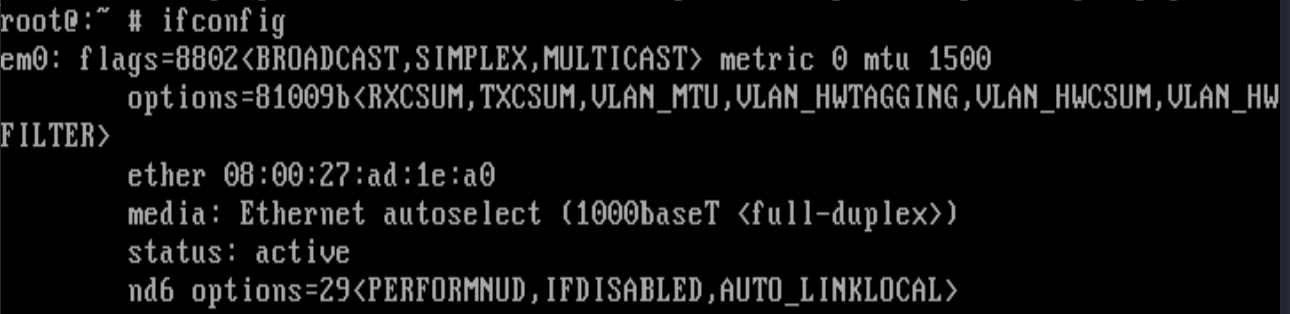
\includegraphics[width=0.90\textwidth]{Interfejs_bez_ip}
  \centering
  \caption{Interfejs bez adresu IPv4}
  \label{fig:if_bez_ip}
\end{figure}

By pobrać adres od serwera DHCP wywołałem komendę \texttt{dhclient em0}.

Następnie wygenerowałem klucze maszyny poleceniem \texttt{ssh-keygen -A} oraz zmieniłem ustawienia demona ssh dodając do pliku \textit{/etc/rc.conf} linię \\ ,, sshd\_enable="YES" ''. Po zakończeniu konfiguracji uruchomiłem serwis poleceniem \texttt{service sshd restart}.

Aby przetestować efekt zalogowałem się z systemu gospodarza poleceniem \texttt{ssh root@192.168.1.126}.

\subsection{Kreacja interfejsów}
Poleceniem \texttt{ifconfig bridge create} utworzyłem wirtualny mostek oraz podłączyłem go do interfejsu em0 poleceniem \texttt{ifconfig bridge0 addm em0}.

Następnie utworzyłem dwie pary interfejsów \textit{e-pair} wywołując dwukrotnie \texttt{ifconfig epair create}. Każdą z tak utworzonych par podłączyłem do mostka wykonując \texttt{ifconfig bridge0 addm epair0a} oraz \texttt{ifconfig bridge0 addm epair1a}.

\paragraph{Efekt wykonanych poleceń} wyświetliłem wywołując \texttt{ifconfig} bez argumentów.

\begin{figure}[H]
  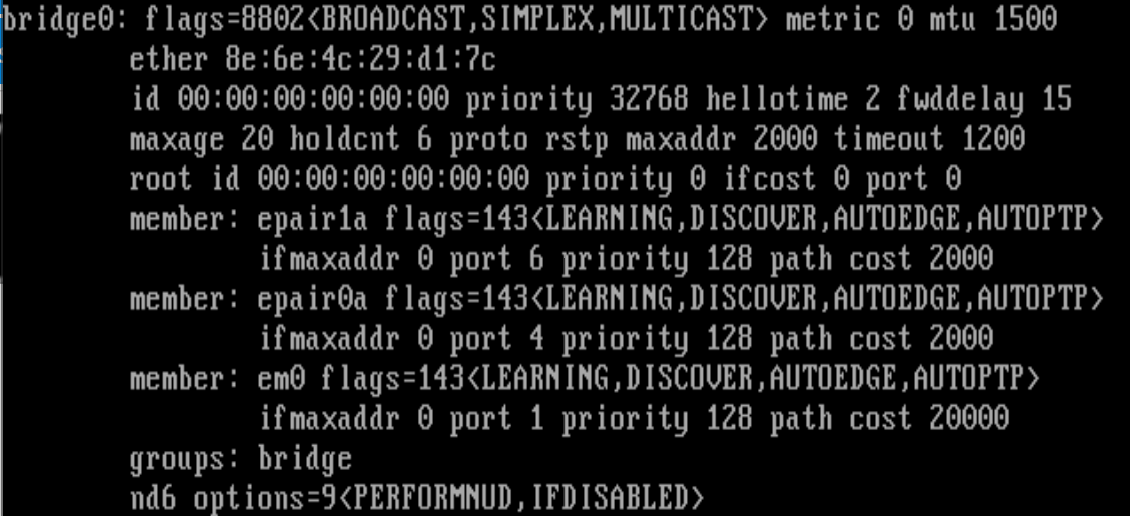
\includegraphics[width=0.90\textwidth]{Podlaczone_interfejsy}
  \centering
  \caption{Gotowa konfiguracja}
  \label{fig:konfiguracja_freebsd}
\end{figure}

\end{document}

